\documentclass[../lab2.tex]{subfiles}

\begin{document}

    \begin{wrapfigure}{r}{0.5\textwidth}
        \vspace{-15pt}
        \centering
        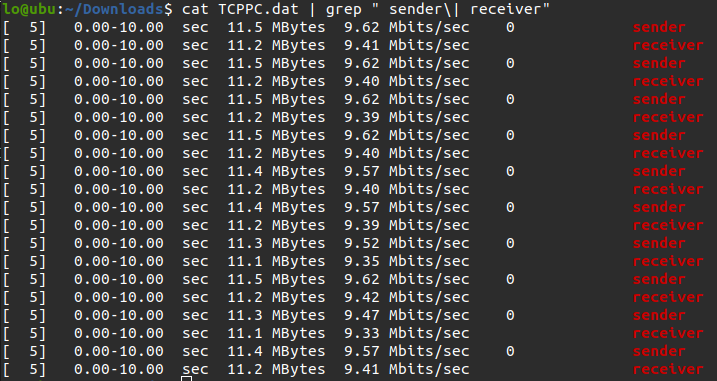
\includegraphics[width=0.5\textwidth]{s&r_conf1.png}
        \caption{}
        \vspace{-25pt}
    \end{wrapfigure}

           Eseguendo il comando si ottiene un riscontro di quanto ipotizzato al punto 
           precedente. In particolare eseguendo 10 test si ottengono i risultati in Figura 1.
           Si può notare che il bitrate del sender è legermente sovrastimato rispetto a quello del 
           receiver: ciò accade perchè i $\Delta T$ di sender e receiver sono differenti, il primo
           calcola il tempo trascorso dall'invio del primo pacchetto all'invio dell'ultimo, mentre il 
           secondo usa tempi più grandi poichè deve attendere la ricezione. 
           Si ottiene quindi una velocità media di 9.58 Mbit/s al sender e 9.39 Mbit/s al receiver.
\vspace{-10pt}
\subsection{Test TCP - Singolo flusso, half duplex}

            In questo caso è possibile predirre l'efficenza della rete tenendo in considerazione il funzionamento di TCP: il protocollo 
            prevede infatti l'invio di un ACK di dimensioni 20+20+38, una volta che il receiver ha ricevuto il pacchetto. 

            \begin{equation}
                \centering
                \eta = \frac{MSS}{MSS+20+32+38+(20 + 20 + 38)}\simeq 0.89
            \end{equation}
            Essendo il canale condiviso per trasmissione e ricezione possono verificarsi collisioni a livello fisico che porterebbero a
            una diminuzione del goodput calcolato. Eseguendo il test si ottengono le seguenti velocità di trasmissione\\
   
               
        
            Come ipotizzato la velocità è piu' lenta di quella calcolata per via delle collisioni, gestite direttamente 
            dalla scheda di rete, visualizzabili con \textit{ifconfig} prima e dopo il comando \textit{iperf3}

\subsection{Test TCP - Singolo fulsso, full duplex, reverse mode}

            \begin{figure}[!htb]
                \begin{minipage}{0.48\textwidth}
                    \centering
                    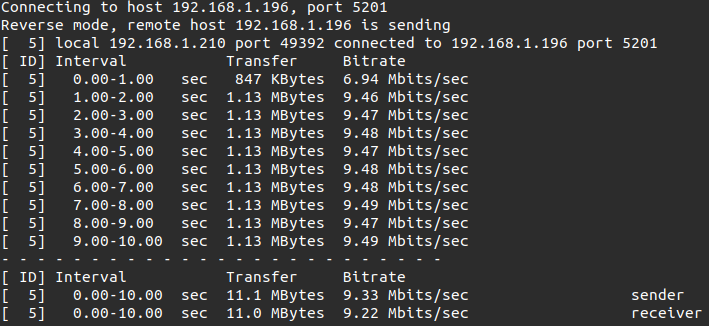
\includegraphics[width=1\linewidth]{PCR.png}
                    \vspace{-20pt}
                    \caption{TCP PC -R}\label{TCPPCR}
                \end{minipage}\hfill
                \begin{minipage}{0.48\textwidth}
                    Facendo riferimento al setup precendente si esegue il comando \textit{iperf3 -c 192.168.1.196 -R}
                    al client, in questo modo è il client a mandare un primo messaggio al server per richiedere la connessione inversa, scambiando così i ruoli 
                    di client e server.
                    In questo scenario la velocità del client è molto maggiore di quella del server, per questo motivo interverranno 
                    il controllo di congestione e di flusso per adattare, nei primi istanti della connessione, la velocità di 
                    \textit{sender} e \textit{receiver} per evitare congestione e ritrasmissioni che diminuirebbero il goodput della rete.
                \end{minipage}
            \end{figure}

            In figura 2 e' possibile notare l'intervento del controllo di congestione guardando la quantita' di dati scambiati nel primo secondo rispetto agli istanti 
            successivi. Eseguendo il comando 10 volte e' possibile ricavare le velocità medie di sender e receiver, rispettivamente 9.33 e 9.20.
            
    \subsection{Test UDP - Singolo flusso, full duplex}

            L'efficenza di UDP è massima se si riescono a scambiare la maggiore quantità di bit senza che avvenga frammentazione del pacchetto,
            ovvero quando $S+8+20 = MTU$, quindi $S_{MAX} = 1472$

            Dalla (2) si ricava che 
            
            \begin{equation}
                \centering
                \eta = \frac{1472}{1472+8+20+38} \simeq 0,957 \rightarrow  V_{TXMAX} = C \cdot \eta = 9,57 Mb/s
            \end{equation}

            Nel caso del singolo flusso full duplex non ci aspettiamo problemi a livello fisico, nè problemi di congestione della rete.
            Poichè UDP è un protocollo inaffidabile e non aspetta conferme dall'interlocutore, l'efficenza per connessioni
            half duplex rimane la stessa di quella calcolata precedentemente.
            La velocità ottenuta risulta essere maggiore di quella TCP per via delle dimensioni ridotte dell'header UDP 

            \subsection{Risultati}

            \begin{figure}[!h]
                \begin{minipage}{0.48\textwidth}
                    \centering
                    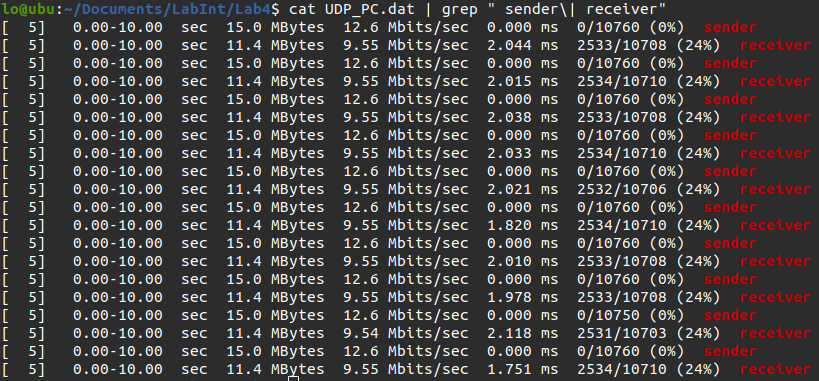
\includegraphics[width=1\linewidth]{UDPsenrec.png}
                    \vspace{-20pt}
                    \caption{UDP PC}\label{UDPPC}
                \end{minipage}\hfill
                \begin{minipage}{0.48\textwidth}
                    A conferma della maggiore efficenza del protocllo UDP eseguendo i 10 test si ottiene una velocità media 
                    di 12.6 al sender e 9.56 al receiver. Poichè non viene limitato il bitrate di generazione dei pacchetti 
                    (opzione \textit{-b 0}) e il sender li genera ad una velocità maggiore di 10 Mb/s una parte 
                    dei pacchetti creata non può essere smaltita dalla pila protocollare del sender, in questo caso il 24\%.
                \end{minipage}
            \end{figure}

            \subsection{Test UDP - Singolo flusso, full duplex, reverse mode}
            \begin{figure}[!htb]
                \begin{minipage}{0.48\textwidth}
                    \centering
                    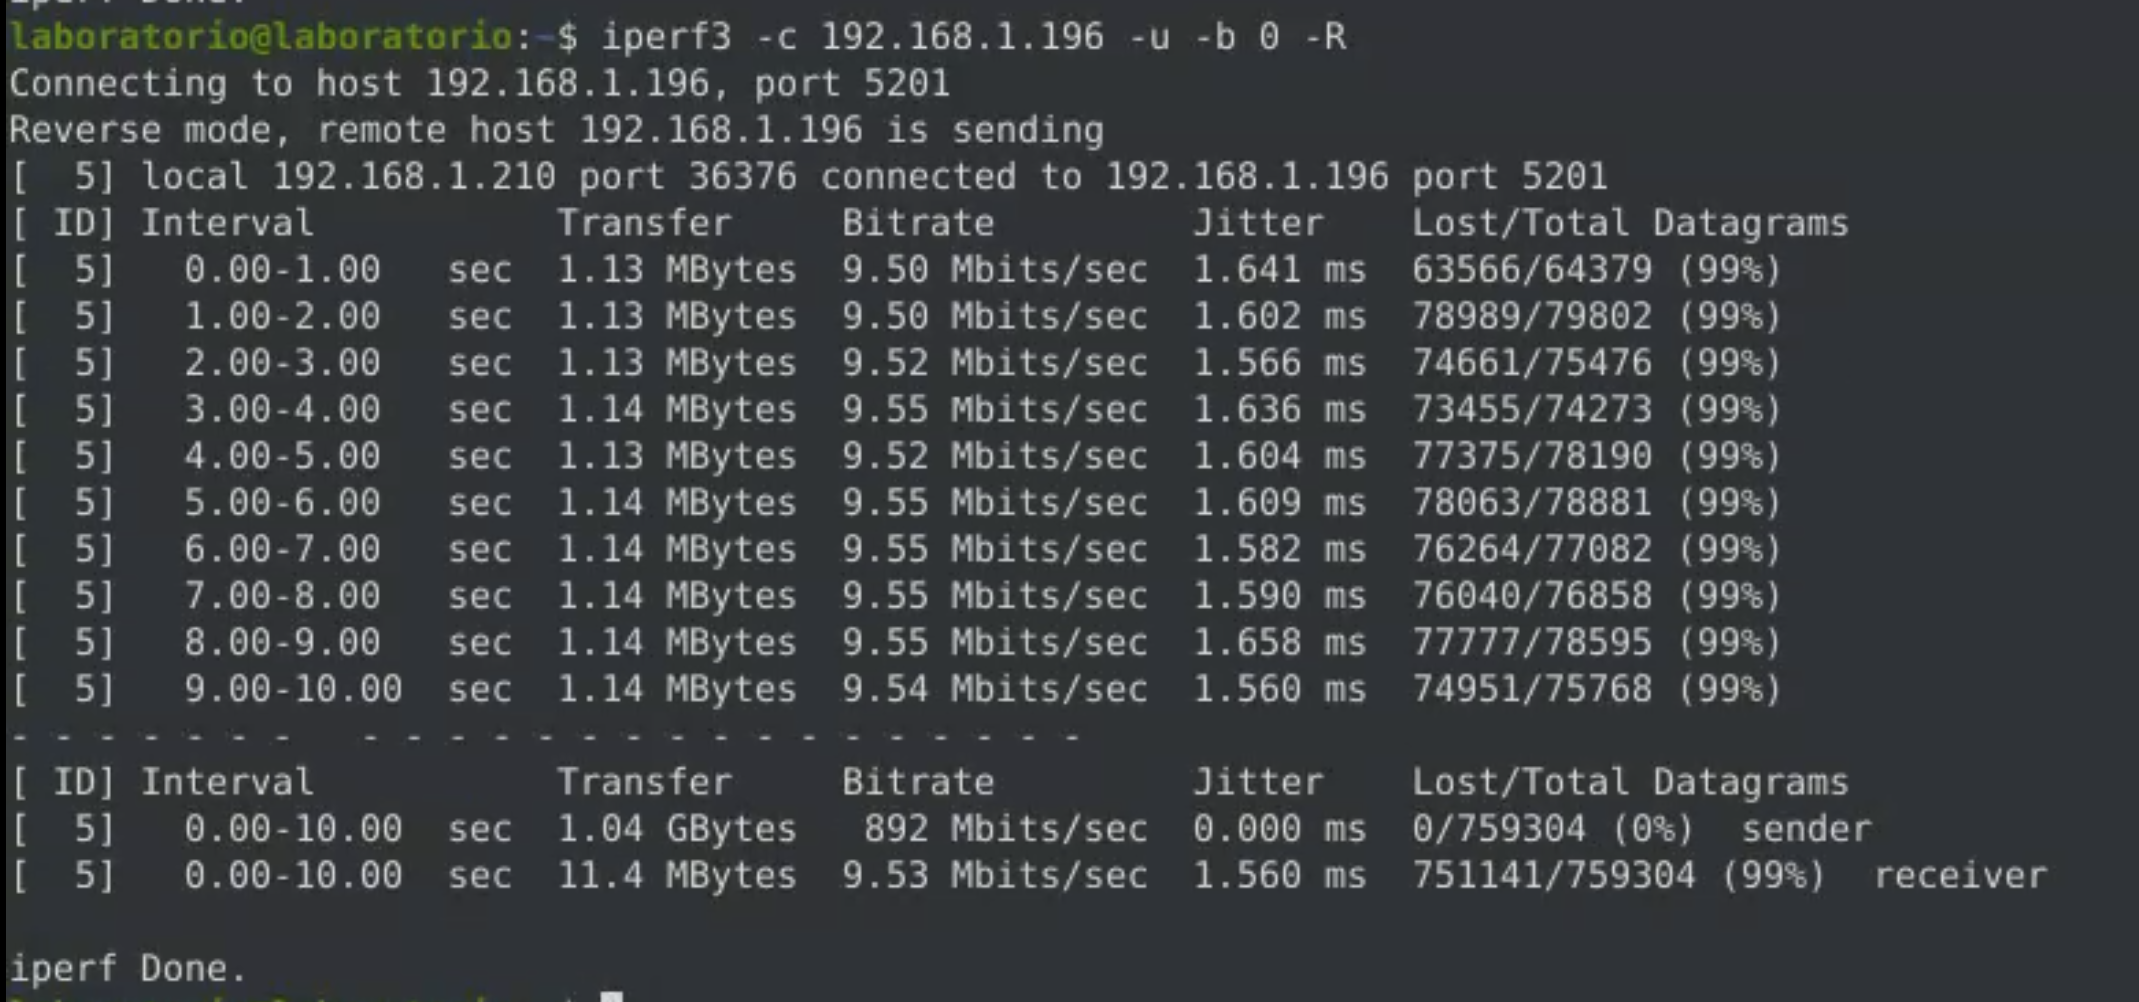
\includegraphics[width=1\linewidth]{UDPrevPC.png}
                    \vspace{-20pt}
                    \caption{UDP PC -R}\label{UDPPCR}
                \end{minipage}\hfill
                \begin{minipage}{0.48\textwidth}
                    Essendo 1000 Mb/s la velocità tra il server e lo switch ci aspettiamo di avere una situazione di \textit{bottleneck} poichè il client riceve solo a 10 Mb/s. Come si puo' notare dalla Figura 4 infatti abbiamo
                    il 99\% di pacchetti persi a causa della congestione della rete dovuta al riempimento della coda presente
                    nello switch.    
                \end{minipage}
            \end{figure}


\end{document}